\section{Evaluation}
\label{sec:eval}
Our experiment is divided into three parts.
The first part evaluates the accuracy of each of the three main components of
the top-$k$ list extraction system. The second part evaluates the time
performance of the system. The third part gives the end-to-end system
accuracy. The first two parts target a smaller dataset
which is described below. And these experiments were
conducted on a PC with \ZZX{4GB} RAM and 2.70GHz Dual-Core Intel CPU.
The third part evaluates our system at a much larger scale of an entire
Bing snapshot on {\em Cosmos}, a large distributed system at Microsoft.

The top-$k$ extraction is a brand new topic in web mining.
Although there have been many previous attempts
to extract general lists and tables from the web, none of them target
on top-$k$ lists and are able to solve this specific problem. Therefore, we
cannot set up any direct comparison with those methods.  Instead,
we compare several versions of our system, to show the significant
improvement against our previous demo system~\cite{ZZX2012KDD}.

In the remainder of the section, we first describe the benchmark
datasets and the knowledge bases that we used in our evaluation.
Then we present the results for the three-part experiment,
before finally showing some interesting properties about the extracted
top-$k$ lists.

\subsection{Datasets and Knowledge Bases}
We created several benchmark datasets to test the various functional modules
of the system. In general, the benchmarks are pages or titles randomly
sampled from the Bing snapshot, and we created several different types of
ground-truth labels for different evaluation purposes (Table \ref{tab:whRes}).

\begin{table}
\centering
\caption{Benchmarks Details}
\begin{tabular}{|c||c|c|c|c|}
\hline
Name& Type & Size & Label Types & \# of Labels\\\hline
\emph{Title-1} & web titles & 5000 & top-$k$ titles & 118\\
\emph{Title-2} & top-$k$ titles & 5000 & when/where info & 403/389\\
\emph{Page-1} & top-$k$ pages & 1000 & top-$k$ list content & 1000\\
\emph{Page-2} & web pages & 1.6B & top-$k$ list content & 2.24M\\
\hline
\end{tabular}

\label{tab:benchmark}
\end{table}

We have two title benchmarks and two page benchmarks.
\emph{Title-1} and \emph{Title-2} are both sampled from a
Bing fragment called $T_2$, different from $T_1$ mentioned in
Section \ref{sec:imp}. {\em Title-1} are general titles which contains
at least a number form.
{\em Title-2} are top-$k$ titles sampled from true positives output by the
Title Classifier.
\emph{Page-1} is a set of randomly sampled top-$k$ pages whose titles are in
{\em Title-2} and whose list content is labeled.
\emph{Page-2} is
%designed to test the performance and scalability of
%the whole system. It is
a set of high-frequency web pages from a Bing snapshot,
1.6 billion in total.
%The expected number of true top-$k$ pages in this set
%is estimated Section \ref{sec:bigdata}.
%
%For title-based tests (\ref{sec:evalTitle} and \ref{sec:evalDate}), we have \emph{Title-1} and \emph{Title-2}.
%The former is a set of general web page titles.
%To guarantee that training data will not appear in this benchmark,
%we randomly collect titles in another fragment of Bing corpus $T_{2}$.
%The ground truth are top-$k$ titles, which are labeled by human-beings.
%\emph{Title-2} is a set of top-$k$ titles with temporal and spacial information manually labeled.
%To obtain so many top-$k$ titles efficiently, we processed $T_{2}$ with current Title Classifier
%and randomly sampled true positives.
%
%We also build two benchmarks of pages, which are \emph{Page-1} and \emph{Page-2}.
%\emph{Page-1} is for list extraction test. It is a set of top-$k$ pages with labeled top-$k$ list content.
%We randomly sampled these pages from top-$k$ pages whose titles are in benchmark \emph{Title-2}.
%\emph{Page-2} is designed to test the performance and scalability of the whole system,
%therefore we the whole high-frequency web snapshot from Bing,
%which contains 1.3 billion general web pages.
%We also estimate the total ground truth (top-$k$ pages), which is specified in \ref{sec:topKSum}.

%
%For page-based test (\ref{sec:evalList} and \ref{sec:bigData}, we build two benchmarks \emph{Page-1} and
%\emph{Page-2}.
%\emph{Page-1} is a set of top-$k$ pages with labeled top-$k$ list content.
%The pages are randomly selected from top-$k$ pages whose titles are in \emph{Title-2}.

%To obtain so many top-$k$ titles efficiently,
%we first process $T_{2}$ with current Title Classifier and manually label true positives
%
%For

In addition, to evaluate the impact of the knowledge base on our system,
we prepare several subsets of Probase concept-instance pairs and
also the complete set of 25,229 hypernym-hyponym pairs from
WordNet \cite{wordnet} to act as different is-a knowledge bases.
The subsets of Probase data is sampled by two methods:
{\em Random} which is randomly sample 20\%, 40\%, 60\% and 80\% of the total
data , and {\em Threshold} which selects
Probase pairs whose frequencies are higher than $n$: $n \in \{ 1, 2, 3, 4 \}$.
The latter method removes rare concept-instance pairs in the ``long tail''.

%In order to evaluate how the quality of the knowledge base affects system performance,
%we generate some Probase subsets using different criteria.
%In addition, we use WordNet\cite{wordnet} as an alternative knowledge base,
%which consists of 25,229 concepts (nouns that have hyponyms or instances).
%Replacing the full Probase with these smaller knowledge bases,
%we conduct contrast experiments for functional components,
%and find that the rich concept space of Probase can effectively advance the performance
%of Title Classifier and List Extractor of the system.
%
%We build two series of Probase subsets using the following criteria:
%1. \emph{Random}: we build four Probase subsets by randomly selecting
%20\%, 40\%, 60\% and 80\% Probase concepts.
%2. \emph{Threshold}: we build four Probase subsets by selecting
%Probase concepts of frequency higher than $n$ ($n \in \{ 1, 2, 3, 4 \}$).
%This method is supposed to filter the ``long tail'' in the concept histogram,
%which are mostly rare concepts or noises.


\subsection{Component Accuracy}
\subsubsection{Title Recognition}
\label{sec:evalTitle}

\ZZX{To test the performance of the CRF model,
we run Title Classifier on \emph{Title-1}.}
The F-measure of the classifier is around 83.5\%
with Precision $\approx76.7\%$ and Recall $=92.4\%$.
The high recall ensures that most of the real top-$k$ pages can pass
through this stage.
\ZZX{Figure \ref{fig:titleProbase} shows that
without any Probase knowledge,
F-measure drops to 74.3\% (Precision $\approx69.6\%$, Recall $=79.7\%$),
which is about 11\% lower than the one with full Probase.
Using the full WordNet as the knowledge base, the accuracy is boosted
by less than 2\% (the red dashed line in Figure \ref{fig:titleProbase}),
which indicates that Probase has some advantage over WordNet at title
recognition due its stronger coverage on multi-word expressions.
We also compare the two subset generating methods,
and conclude that the \emph{threshold} method is relatively better,
because the knowledge thus created is of better quality.
}

\subsubsection{Date and Location Detection}
\label{sec:evalDate}
%In this subsection we test the accuracy performance of date and location detection function.
%We build a benchmark with 1000 ``top-$k$ like'' titles.
We test the accuracy performance of date and location detection function,
using a benchmark \emph{Title-2}.
In {\em Title-2}, 736 titles are verified to have
temporal or spacial information, of which 403 contain date information
and 389 contain location information.
The results of detection are shown in Table \ref{tab:whRes}.
%We use the detector to process the benchmark, the result is shown in Table \ref{tab:whRes}.

\begin{table}
\centering
\caption{Results for Date and Location Detection}
\begin{tabular}{|c||c|c|c|}
\hline
Type  & Precision & Recall &  F-measure \\\hline
Date  & 83.3\% & 94.4\% & 88.3\%\\
Location & 85.8\% & 82.5\% & 84.1\%\\
\hline
\end{tabular}

\label{tab:whRes}
\end{table}

\subsubsection{List Extraction}

\label{sec:evalList}

Since HTML Parser, Candidate Picker and Top-K Ranker all
contribute to list extraction, we put them together as one functional
unit and test its accuracy.
We run the whole system on \emph{Page-1}.
As the titles in \emph{Page-1} come from \emph{Title-2},
they are guaranteed to be recognized correctly,
thus eliminating the effect of the Title Classifier.

The result is shown in Table \ref{tab:listRes},
where we compare the two ranking algorithms.
%In this table, we also list the result for the two algorithms of the original system\cite{ZZX2012KDD}.
%We can see that, the current system has the highest F-measure among the three versions.
We can see that the \emph{learning-based} ranker generally performs
better than the \emph{rule-based} approach in both precision and
recall. This advantage becomes more apparent in the
end-to-end experiments on big data later.
%In addition, the amount of
%knowledge appears to have lesser positive impact on the accuracy
%in learning-based approach than rule-based. \KZ{Why??}

Also, we evaluate the impact of knowledge base quality with
different Probase subsets as well as the WordNet,
shown in Figure \ref{fig:listProbase}.
First, subsets produced by \emph{threshold} methods yield better results
than \emph{random} subsets.
Second, without Probase knowledge,
the performance of \emph{rule-based} ranker drops dramatically
(from 82.0\% to 72.3\%), while \emph{learning-based} ranker is
less affected (from 86.8\% to 83.5\%).
This is because (1) \emph{learning-based} ranker uses many more features
than the \emph{rule-based} ranker;
and (2) the model of \emph{learning-based} ranker is adaptive to
the reduced quality of Probase (by adjusting feature weight).

\begin{table}
\centering
\caption{Results for List Extraction}
\begin{tabular}{|c||c|c|c|}
\hline
Algo  & Precision & Recall & F-measure\\\hline
%Default  & 89.3\% & 83.5\% & 86.3\% \\
Rule-based  & 95.5\% & 71.9\% & 82.0\% \\
\textbf{Learning-based}  & \textbf{97.5\%} & \textbf{78.2\%} & \textbf{86.8\%}\\
\hline
\end{tabular}
\label{tab:listRes}
\end{table}

\subsection{Time Performance}

%When running the system on \emph{Page-1},
%we also record the running time of each step to evaluate system efficiency.
On average, the system takes 109 ms to process one page on {\em Page-1}.
Most of that time is consumed by the HTML parser (67 ms). The main algorithm,
including Candidate Picker, Top-K Ranker and Content Processor,
only takes about 1/3 of total running time (36 ms).
In addition, if Title Classifier returns negative for a non-top-$k$ page,
the system immediately returns, in which case, only 6 ms is needed.

Figure \ref{fig:FileSize} plots the average running time of each page versus
the page file size over 10 runs, which indicated near-linear
scalability in file sizes.


%Also, we conduct a scaling test of file size
%on \emph{Page-1}.
%The result is shown in Figure \ref{fig:FileSize},
%in which the x-axis represents the
%file size of tested pages,
%while the y-axis means the corresponding running time.
%This figure shows that the system has a near-linear scalability in file size.

\begin{figure*}[th]
\centering
\subfigure[Title Recognition with Probase subsets]{
  \label{fig:titleProbase}
  \epsfig{file=./pics/titleProbase.eps,width=0.645\columnwidth}
}
\subfigure[List Extraction with Probase subsets]{
  \label{fig:listProbase}
  \epsfig{file=./pics/listExtractionProbase.eps,width=0.645\columnwidth}
}
\subfigure[Scaling Test of File Size]{
  \label{fig:FileSize}
  \epsfig{file=./pics/filesize.eps,width=0.645\columnwidth}
}
\subfigure[The Performance for Big Data]{
  \label{fig:big}
  \epsfig{file=./pics/bigdata.eps,width=0.645\columnwidth}
}
\subfigure[The Distribution of Number K]{
  \label{fig:kDistri}
  \epsfig{file=./pics/k_distribute.eps,width=0.645\columnwidth}
}
\subfigure[The Distribution of Number of Attributes]{
  \label{fig:colDistri}
  \epsfig{file=./pics/col_distribute.eps,width=0.645\columnwidth}
}
\caption{Experimental Results}
\label{fig:results}
\end{figure*}

%\begin{figure}[th]
%	\centering
%	\epsfig{file=./pics/filesize.eps,width=0.9\columnwidth}
%	\caption{Scaling Test of File Size}
%	\label{fig:FileSize}
%\end{figure}

\subsection{End-to-end Evaluation}
\label{sec:bigdata}
%In our demo paper, we have estimated the sum of top-$k$ pages.
%We sampled 1000 normal web pages and find 14 top-$k$ pages.
%Thus the total number should be $1.4\textperthousand \times 1,600,000,000 \approx 2,240,000$
%(assuming that there are 1.6 billion web pages in total).

Before we conduct the experiment on Bing snapshot (\emph{Page-2}),
we estimate the total number of top-$k$ pages
to calculate the system recall.
\ZZX{
We first use Title Classifier to identify a subset of \emph{Page-2}.
which contains 1.6 million pages (1/1000 of \emph{Page-2}).
The classifier recognizes 5,994 pages from the subset.
2,061 of them are manually verified to be real top-$k$ pages.
Considering that 7.6\% of the pages are missed by the classifier,
the total number of top-$k$ pages should be about 2,231.
Therefore the expected number of top-$k$ pages in \emph{Page-2}
is approximately 2,231,000, which is about 1.4\textperthousand.
}

%As we need to calculate the recall for the overall system,
%we must estimate the total number of top-$k$ pages.
%Known that the recall of the title classifier is 92\%,
%we use it to identify 1.6 million pages
%(about 1/1000 of total pages in the web), and obtain 5994 pages.
%By manually check these pages,
%we find 2,061 of them are real top-$k$ pages.
%Considering there are 8\% missed by the classifier,
%the total number of top-$k$ pages should be $2,061\div92\%\approx2,240$.
%Therefore the total number of top-$k$ pages should be approximately $2,240\times1,000=2,240,000$.
%Assuming that there are 1.6 billion web pages in total, the proportion of top-$k$ pages are $2,240,000 \div 1,600,000,000\approx0.0014=1.4$\textperthousand.

The end-to-end experiment aims to show: 1) the overall system performance on
real web pages; and 2) the total number of top-$k$ lists that can be extracted
from the entire web.
%First is to test the system's overall performance,
%and show that our system works for the real-world web pages;
%second is to extract as many top-$k$ lists as possible from the entire web.
To this end, the system extracted 1,753,124 top-$k$ lists from {\em Page-2}.
Random sample of 1000 lists from the extracted result
has a precision of 92.0\%. If we project this result up to the whole of
{\em Page-2}, we should have extracted 1,612,874 top-$k$ in total,
and the estimated recall is 72.3\%.

We compare the \emph{rule-based} and \emph{learning-based} algorithms for
processing big data in Figure \ref{fig:big}.
\emph{Rule-based} algorithm attains 90.4\% precision and 57.9\% recall which
is outperformed by the {\em learning-based} algorithms (the default algorithms) 
reported above.
%It is apparent that the learning-based algorithm is better in both
%scores.
%Especially, the current system shows significant improvement
%in the recall,
Learning-based algorithms have a clear advantage in recall which results in
300,000 more top-$k$ lists extracted from the whole web.

\subsection{Some Properties of Top-$k$ Lists}
%With the result data we obtained from the experiments above,
%we do some analysis and find some interesting features about top-$k$ lists.
In the following experiments, we create a test set of
100,000 randomly sampled lists from the result of the big data experiment.

\subsubsection{Distribution of $K$}
The first experiment studies the distribution of the number $k$.
The system imposes a constraint of $2 \le k \le 5000$.
In our sample, the largest $k$ equals to 4,526.
Figure \ref{fig:kDistri} shows the distribution for $2 \le k \le 35$.
From this figure, multiples of 5 and 10 are more popular than their neighbors.
In particular, 5 and 10 are two most popular numbers, which
make up 65\% of all occurrences.
For the other numbers, the frequency generally decreases as the $k$ grows.

%The experimental result is consistent with our common sense.
%The editors of top-$k$ pages prefer to use a multiple of 5 or 10 as $k$,
%since it is easier to remember.
%And generally they may not choose a too large number
%since it is difficult to place all list items into a single page.

%\begin{figure}[th]
%	\centering
%	\epsfig{file=./pics/k_distribute.eps,width=\columnwidth}
%\caption{The Distribution of Number K}
%\label{fig:kDistri}
%\end{figure}

\subsubsection{Distribution in Number of Attributes}
Figure \ref{fig:colDistri} shows the distribution of number of
attributes (columns) in the extracted list content (with a cut-off at 20).
In the test set, the largest number of attributes is 62.
Most of the top-$k$ lists contain 2 or 3 attributes.
The frequency decreases as the column number grows.

%\begin{figure}[th]
%	\centering
%	\epsfig{file=./pics/col_distribute.eps,width=\columnwidth}
%\caption{The Distribution of Column Number}
%\label{fig:colDistri}
%\end{figure}
\subsubsection{Percentage of Ranked Top-$k$ Lists}
\label{sec:rankedlist}
By detecting an indexing pattern, we find 63,212 lists with explicit ranking information, 
which indicates 63.2\% of top-$k$ lists are ranked.

